\section{Observation and Calculations}
Least count of the instrument = 0.5 V.
Using data from table \ref{tab}, we have plotted $I_C$ vs. $U_A$ for 3 different datasets as follows.

\begin{figure}[H]
    \centering
    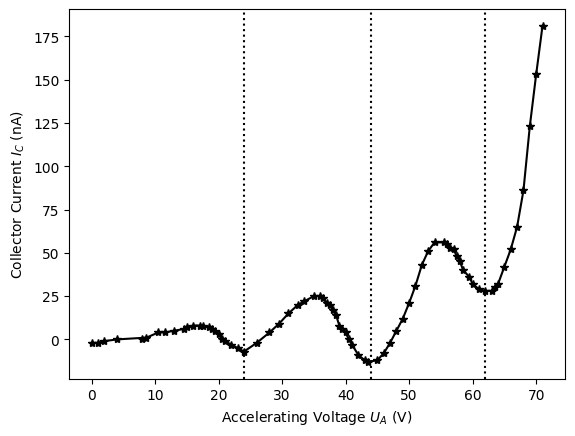
\includegraphics[width=1\columnwidth]{images/g1.png}
    \caption{$I_C$ vs. $U_A$ for $U_F = 8.5$ V, $U_{G} = 4$ V, $U_E=4$ V}
    \label{g1}
\end{figure}

\noindent From the first 2 minima, $\Delta U_1=(20.0 \pm 0.5)$  V\\
From the 2nd and 3rd minima $\Delta U_2=(18.0 \pm 0.5)$ V\\
So, $\Delta U_\text{avg}$ = $(19.0 \pm 0.4)$ V

\begin{figure}[H]
    \centering
    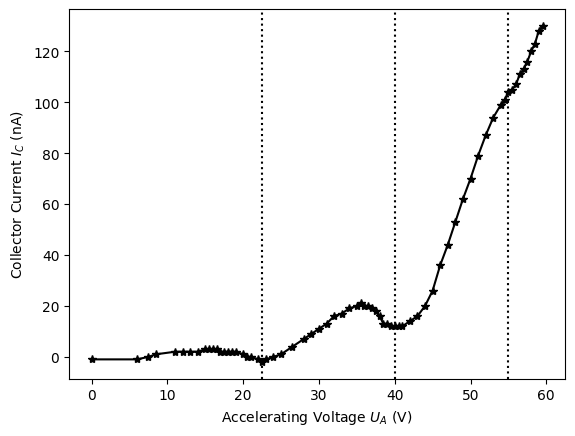
\includegraphics[width=1\columnwidth]{images/g3.png}
    \caption{$I_C$ vs. $U_A$ for $U_F = 8.5$ V, $U_{G} = 4.8$ V, $U_E=5$ V}
    \label{g3}
\end{figure}

\noindent From the first 2 minima, $\Delta U_1=(17.5 \pm 0.5)$  V\\
From the 2nd and 3rd minima $\Delta U_2=(15.0 \pm 0.5)$ V\\
So, $\Delta U_\text{avg}$ = $(16.3 \pm 0.4)$ V

\begin{figure}[H]
    \centering
    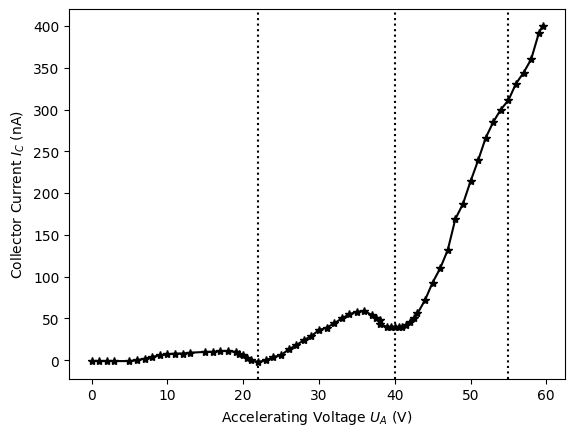
\includegraphics[width=1\columnwidth]{images/g2.png}
    \caption{$I_C$ vs. $U_A$ for $U_F = 8.5$ V, $U_{G} = 5$ V, $U_E=4.5$ V}
    \label{g2}
\end{figure}

\noindent From the first 2 minima, $\Delta U_1=(18.0 \pm 0.5)$  V\\
From the 2nd and 3rd minima $\Delta U_2=(15.0 \pm 0.5)$ V\\
So, $\Delta U_\text{avg}$ = $(16.5 \pm 0.4)$ V

\begin{table*}
\begin{ruledtabular}
    \begin{tabular}{|cccccccccc|}
        \multicolumn{1}{|c|}{$U_A$ (V)} & \multicolumn{1}{c|}{$I_C$ (nA)} & \multicolumn{1}{c|}{$U_A$ (V)} & \multicolumn{1}{c|}{$I_C$ (nA)} & \multicolumn{1}{c|}{$U_A$ (V)} & \multicolumn{1}{c|}{$I_C$ (nA)} & \multicolumn{1}{c|}{$U_A$ (V)} & \multicolumn{1}{c|}{$I_C$ (nA)} & \multicolumn{1}{c|}{$U_A$ (V)} & $I_C$ (nA) \\ \hline
        \multicolumn{10}{|c|}{$U_F = 8.5$ V,   $U_{G} = 4$ V, $U_E=4$ V}                                                                                                                                                                                                                                                         \\ \hline
        \multicolumn{1}{|c|}{0.0}       & \multicolumn{1}{c|}{-2}         & \multicolumn{1}{c|}{20.0}      & \multicolumn{1}{c|}{3}          & \multicolumn{1}{c|}{38.0}      & \multicolumn{1}{c|}{17}         & \multicolumn{1}{c|}{52.0}      & \multicolumn{1}{c|}{43}         & \multicolumn{1}{c|}{65.0}      & 42         \\ \hline
        \multicolumn{1}{|c|}{1.0}       & \multicolumn{1}{c|}{-2}         & \multicolumn{1}{c|}{20.5}      & \multicolumn{1}{c|}{0}          & \multicolumn{1}{c|}{38.5}      & \multicolumn{1}{c|}{14}         & \multicolumn{1}{c|}{53.0}      & \multicolumn{1}{c|}{51}         & \multicolumn{1}{c|}{66.0}      & 52         \\ \hline
        \multicolumn{1}{|c|}{2.0}       & \multicolumn{1}{c|}{-1}         & \multicolumn{1}{c|}{21.0}      & \multicolumn{1}{c|}{-1}         & \multicolumn{1}{c|}{39.0}      & \multicolumn{1}{c|}{8}          & \multicolumn{1}{c|}{54.0}      & \multicolumn{1}{c|}{56}         & \multicolumn{1}{c|}{67.0}      & 65         \\ \hline
        \multicolumn{1}{|c|}{4.0}       & \multicolumn{1}{c|}{0}          & \multicolumn{1}{c|}{22.0}      & \multicolumn{1}{c|}{-3}         & \multicolumn{1}{c|}{39.5}      & \multicolumn{1}{c|}{6}          & \multicolumn{1}{c|}{55.5}      & \multicolumn{1}{c|}{56}         & \multicolumn{1}{c|}{68.0}      & 86         \\ \hline
        \multicolumn{1}{|c|}{8.5}       & \multicolumn{1}{c|}{1}          & \multicolumn{1}{c|}{23.0}      & \multicolumn{1}{c|}{-5}         & \multicolumn{1}{c|}{40.0}      & \multicolumn{1}{c|}{4}          & \multicolumn{1}{c|}{56.0}      & \multicolumn{1}{c|}{55}         & \multicolumn{1}{c|}{69.0}      & 123        \\ \hline
        \multicolumn{1}{|c|}{8.0}       & \multicolumn{1}{c|}{0}          & \multicolumn{1}{c|}{24.0}      & \multicolumn{1}{c|}{-7}         & \multicolumn{1}{c|}{40.5}      & \multicolumn{1}{c|}{0}          & \multicolumn{1}{c|}{56.5}      & \multicolumn{1}{c|}{53}         & \multicolumn{1}{c|}{70.0}      & 153        \\ \hline
        \multicolumn{1}{|c|}{10.5}      & \multicolumn{1}{c|}{4}          & \multicolumn{1}{c|}{26.0}      & \multicolumn{1}{c|}{-2}         & \multicolumn{1}{c|}{41.0}      & \multicolumn{1}{c|}{-3}         & \multicolumn{1}{c|}{57.0}      & \multicolumn{1}{c|}{52}         & \multicolumn{1}{c|}{71.0}      & 181        \\ \hline
        \multicolumn{1}{|c|}{11.5}      & \multicolumn{1}{c|}{4}          & \multicolumn{1}{c|}{28.0}      & \multicolumn{1}{c|}{4}          & \multicolumn{1}{c|}{42.0}      & \multicolumn{1}{c|}{-9}         & \multicolumn{1}{c|}{57.5}      & \multicolumn{1}{c|}{48}         & \multicolumn{1}{c|}{72.0}      & 208        \\ \hline
        \multicolumn{1}{|c|}{13.0}      & \multicolumn{1}{c|}{5}          & \multicolumn{1}{c|}{29.5}      & \multicolumn{1}{c|}{9}          & \multicolumn{1}{c|}{43.0}      & \multicolumn{1}{c|}{-12}        & \multicolumn{1}{c|}{58.0}      & \multicolumn{1}{c|}{45}         & \multicolumn{1}{c|}{73.0}      & 245        \\ \hline
        \multicolumn{1}{|c|}{14.5}      & \multicolumn{1}{c|}{6}          & \multicolumn{1}{c|}{31.0}      & \multicolumn{1}{c|}{15}         & \multicolumn{1}{c|}{43.5}      & \multicolumn{1}{c|}{-13}        & \multicolumn{1}{c|}{58.5}      & \multicolumn{1}{c|}{40}         & \multicolumn{1}{c|}{74.0}      & 271        \\ \hline
        \multicolumn{1}{|c|}{15.0}      & \multicolumn{1}{c|}{7}          & \multicolumn{1}{c|}{32.5}      & \multicolumn{1}{c|}{20}         & \multicolumn{1}{c|}{45.0}      & \multicolumn{1}{c|}{-12}        & \multicolumn{1}{c|}{59.5}      & \multicolumn{1}{c|}{36}         & \multicolumn{1}{c|}{75.0}      & 315        \\ \hline
        \multicolumn{1}{|c|}{16.0}      & \multicolumn{1}{c|}{8}          & \multicolumn{1}{c|}{33.5}      & \multicolumn{1}{c|}{22}         & \multicolumn{1}{c|}{46.0}      & \multicolumn{1}{c|}{-8}         & \multicolumn{1}{c|}{60.0}      & \multicolumn{1}{c|}{32}         & \multicolumn{1}{c|}{76.0}      & 351        \\ \hline
        \multicolumn{1}{|c|}{17.0}      & \multicolumn{1}{c|}{8}          & \multicolumn{1}{c|}{35.0}      & \multicolumn{1}{c|}{25}         & \multicolumn{1}{c|}{47.0}      & \multicolumn{1}{c|}{-2}         & \multicolumn{1}{c|}{61.0}      & \multicolumn{1}{c|}{29}         & \multicolumn{1}{c|}{77.0}      & 399        \\ \hline
        \multicolumn{1}{|c|}{17.5}      & \multicolumn{1}{c|}{8}          & \multicolumn{1}{c|}{36.0}      & \multicolumn{1}{c|}{25}         & \multicolumn{1}{c|}{48.0}      & \multicolumn{1}{c|}{5}          & \multicolumn{1}{c|}{62.0}      & \multicolumn{1}{c|}{28}         & \multicolumn{1}{c|}{78.0}      & 400        \\ \hline
        \multicolumn{1}{|c|}{18.5}      & \multicolumn{1}{c|}{7}          & \multicolumn{1}{c|}{36.5}      & \multicolumn{1}{c|}{24}         & \multicolumn{1}{c|}{49.0}      & \multicolumn{1}{c|}{12}         & \multicolumn{1}{c|}{63.0}      & \multicolumn{1}{c|}{28}         & \multicolumn{1}{c|}{80.0}      & 400        \\ \hline
        \multicolumn{1}{|c|}{19.0}      & \multicolumn{1}{c|}{6}          & \multicolumn{1}{c|}{37.0}      & \multicolumn{1}{c|}{21}         & \multicolumn{1}{c|}{50.0}      & \multicolumn{1}{c|}{21}         & \multicolumn{1}{c|}{63.5}      & \multicolumn{1}{c|}{30}         & \multicolumn{1}{c|}{}          &            \\ \hline
        \multicolumn{1}{|c|}{19.5}      & \multicolumn{1}{c|}{5}          & \multicolumn{1}{c|}{37.5}      & \multicolumn{1}{c|}{20}         & \multicolumn{1}{c|}{51.0}      & \multicolumn{1}{c|}{31}         & \multicolumn{1}{c|}{64.0}      & \multicolumn{1}{c|}{32}         & \multicolumn{1}{c|}{}          &            \\ \hline
        \multicolumn{10}{|c|}{$U_F = 8.5$ V,   $U_{G} = 4.8$ V, $U_E=5$ V}                                                                                                                                                                                                                                                       \\ \hline
        \multicolumn{1}{|c|}{0.0}       & \multicolumn{1}{c|}{-1}         & \multicolumn{1}{c|}{16.0}      & \multicolumn{1}{c|}{10}         & \multicolumn{1}{c|}{28.0}      & \multicolumn{1}{c|}{24}         & \multicolumn{1}{c|}{39.5}      & \multicolumn{1}{c|}{40}         & \multicolumn{1}{c|}{50.0}      & 214        \\ \hline
        \multicolumn{1}{|c|}{1.0}       & \multicolumn{1}{c|}{-1}         & \multicolumn{1}{c|}{17.0}      & \multicolumn{1}{c|}{11}         & \multicolumn{1}{c|}{29.0}      & \multicolumn{1}{c|}{29}         & \multicolumn{1}{c|}{40.0}      & \multicolumn{1}{c|}{40}         & \multicolumn{1}{c|}{51.0}      & 239        \\ \hline
        \multicolumn{1}{|c|}{2.0}       & \multicolumn{1}{c|}{-1}         & \multicolumn{1}{c|}{18.0}      & \multicolumn{1}{c|}{11}         & \multicolumn{1}{c|}{30.0}      & \multicolumn{1}{c|}{36}         & \multicolumn{1}{c|}{40.5}      & \multicolumn{1}{c|}{40}         & \multicolumn{1}{c|}{52.0}      & 266        \\ \hline
        \multicolumn{1}{|c|}{3.0}       & \multicolumn{1}{c|}{-1}         & \multicolumn{1}{c|}{19.0}      & \multicolumn{1}{c|}{10}         & \multicolumn{1}{c|}{31.0}      & \multicolumn{1}{c|}{39}         & \multicolumn{1}{c|}{41.0}      & \multicolumn{1}{c|}{40}         & \multicolumn{1}{c|}{53.0}      & 285        \\ \hline
        \multicolumn{1}{|c|}{5.0}       & \multicolumn{1}{c|}{-1}         & \multicolumn{1}{c|}{19.5}      & \multicolumn{1}{c|}{8}          & \multicolumn{1}{c|}{32.0}      & \multicolumn{1}{c|}{44}         & \multicolumn{1}{c|}{41.5}      & \multicolumn{1}{c|}{42}         & \multicolumn{1}{c|}{54.0}      & 300        \\ \hline
        \multicolumn{1}{|c|}{6.0}       & \multicolumn{1}{c|}{0}          & \multicolumn{1}{c|}{20.0}      & \multicolumn{1}{c|}{6}          & \multicolumn{1}{c|}{33.0}      & \multicolumn{1}{c|}{50}         & \multicolumn{1}{c|}{42.0}      & \multicolumn{1}{c|}{46}         & \multicolumn{1}{c|}{55.0}      & 311        \\ \hline
        \multicolumn{1}{|c|}{7.0}       & \multicolumn{1}{c|}{2}          & \multicolumn{1}{c|}{20.5}      & \multicolumn{1}{c|}{3}          & \multicolumn{1}{c|}{34.0}      & \multicolumn{1}{c|}{55}         & \multicolumn{1}{c|}{42.5}      & \multicolumn{1}{c|}{50}         & \multicolumn{1}{c|}{56.0}      & 331        \\ \hline
        \multicolumn{1}{|c|}{8.0}       & \multicolumn{1}{c|}{4}          & \multicolumn{1}{c|}{21.0}      & \multicolumn{1}{c|}{0}          & \multicolumn{1}{c|}{35.0}      & \multicolumn{1}{c|}{58}         & \multicolumn{1}{c|}{43.0}      & \multicolumn{1}{c|}{56}         & \multicolumn{1}{c|}{57.0}      & 344        \\ \hline
        \multicolumn{1}{|c|}{9.0}       & \multicolumn{1}{c|}{6}          & \multicolumn{1}{c|}{22.0}      & \multicolumn{1}{c|}{-2}         & \multicolumn{1}{c|}{36.0}      & \multicolumn{1}{c|}{59}         & \multicolumn{1}{c|}{44.0}      & \multicolumn{1}{c|}{72}         & \multicolumn{1}{c|}{58.0}      & 360        \\ \hline
        \multicolumn{1}{|c|}{10.0}      & \multicolumn{1}{c|}{7}          & \multicolumn{1}{c|}{23.0}      & \multicolumn{1}{c|}{0}          & \multicolumn{1}{c|}{37.0}      & \multicolumn{1}{c|}{54}         & \multicolumn{1}{c|}{45.0}      & \multicolumn{1}{c|}{93}         & \multicolumn{1}{c|}{59.0}      & 391        \\ \hline
        \multicolumn{1}{|c|}{11.0}      & \multicolumn{1}{c|}{8}          & \multicolumn{1}{c|}{24.0}      & \multicolumn{1}{c|}{4}          & \multicolumn{1}{c|}{37.5}      & \multicolumn{1}{c|}{51}         & \multicolumn{1}{c|}{46.0}      & \multicolumn{1}{c|}{110}        & \multicolumn{1}{c|}{59.5}      & 400        \\ \hline
        \multicolumn{1}{|c|}{12.0}      & \multicolumn{1}{c|}{8}          & \multicolumn{1}{c|}{25.0}      & \multicolumn{1}{c|}{6}          & \multicolumn{1}{c|}{38.0}      & \multicolumn{1}{c|}{48}         & \multicolumn{1}{c|}{47.0}      & \multicolumn{1}{c|}{132}        & \multicolumn{1}{c|}{60.0}      & 400        \\ \hline
        \multicolumn{1}{|c|}{13.0}      & \multicolumn{1}{c|}{9}          & \multicolumn{1}{c|}{26.0}      & \multicolumn{1}{c|}{13}         & \multicolumn{1}{c|}{38.0}      & \multicolumn{1}{c|}{43}         & \multicolumn{1}{c|}{48.0}      & \multicolumn{1}{c|}{169}        & \multicolumn{1}{c|}{}          &            \\ \hline
        \multicolumn{1}{|c|}{15.0}      & \multicolumn{1}{c|}{10}         & \multicolumn{1}{c|}{27.0}      & \multicolumn{1}{c|}{18}         & \multicolumn{1}{c|}{39.0}      & \multicolumn{1}{c|}{40}         & \multicolumn{1}{c|}{49.0}      & \multicolumn{1}{c|}{187}        & \multicolumn{1}{c|}{}          &            \\ \hline
        \multicolumn{10}{|c|}{$U_F = 8.5$ V,   $U_{G} = 5$ V, $U_E=4.5$ V}                                                                                                                                                                                                                                                       \\ \hline
        \multicolumn{1}{|c|}{0.0}       & \multicolumn{1}{c|}{-1}         & \multicolumn{1}{c|}{20.0}      & \multicolumn{1}{c|}{1}          & \multicolumn{1}{c|}{35.5}      & \multicolumn{1}{c|}{21}         & \multicolumn{1}{c|}{47.0}      & \multicolumn{1}{c|}{44}         & \multicolumn{1}{c|}{59.0}      & 128        \\ \hline
        \multicolumn{1}{|c|}{6.0}       & \multicolumn{1}{c|}{-1}         & \multicolumn{1}{c|}{20.5}      & \multicolumn{1}{c|}{0}          & \multicolumn{1}{c|}{36.0}      & \multicolumn{1}{c|}{20}         & \multicolumn{1}{c|}{48.0}      & \multicolumn{1}{c|}{53}         & \multicolumn{1}{c|}{59.5}      & 130        \\ \hline
        \multicolumn{1}{|c|}{7.5}       & \multicolumn{1}{c|}{0}          & \multicolumn{1}{c|}{21.0}      & \multicolumn{1}{c|}{0}          & \multicolumn{1}{c|}{36.5}      & \multicolumn{1}{c|}{20}         & \multicolumn{1}{c|}{49.0}      & \multicolumn{1}{c|}{62}         & \multicolumn{1}{c|}{60.0}      & 137        \\ \hline
        \multicolumn{1}{|c|}{8.5}       & \multicolumn{1}{c|}{1}          & \multicolumn{1}{c|}{22.0}      & \multicolumn{1}{c|}{-1}         & \multicolumn{1}{c|}{37.0}      & \multicolumn{1}{c|}{19}         & \multicolumn{1}{c|}{50.0}      & \multicolumn{1}{c|}{70}         & \multicolumn{1}{c|}{61.0}      & 148        \\ \hline
        \multicolumn{1}{|c|}{11.0}      & \multicolumn{1}{c|}{2}          & \multicolumn{1}{c|}{22.5}      & \multicolumn{1}{c|}{-2}         & \multicolumn{1}{c|}{37.5}      & \multicolumn{1}{c|}{18}         & \multicolumn{1}{c|}{51.0}      & \multicolumn{1}{c|}{79}         & \multicolumn{1}{c|}{62.0}      & 165        \\ \hline
        \multicolumn{1}{|c|}{12.0}      & \multicolumn{1}{c|}{2}          & \multicolumn{1}{c|}{23.0}      & \multicolumn{1}{c|}{-1}         & \multicolumn{1}{c|}{38.0}      & \multicolumn{1}{c|}{16}         & \multicolumn{1}{c|}{52.0}      & \multicolumn{1}{c|}{87}         & \multicolumn{1}{c|}{63.0}      & 177        \\ \hline
        \multicolumn{1}{|c|}{13.0}      & \multicolumn{1}{c|}{2}          & \multicolumn{1}{c|}{24.0}      & \multicolumn{1}{c|}{0}          & \multicolumn{1}{c|}{38.5}      & \multicolumn{1}{c|}{13}         & \multicolumn{1}{c|}{53.0}      & \multicolumn{1}{c|}{94}         & \multicolumn{1}{c|}{64.5}      & 202        \\ \hline
        \multicolumn{1}{|c|}{14.0}      & \multicolumn{1}{c|}{2}          & \multicolumn{1}{c|}{25.0}      & \multicolumn{1}{c|}{1}          & \multicolumn{1}{c|}{39.0}      & \multicolumn{1}{c|}{13}         & \multicolumn{1}{c|}{54.0}      & \multicolumn{1}{c|}{99}         & \multicolumn{1}{c|}{65.0}      & 226        \\ \hline
        \multicolumn{1}{|c|}{15.0}      & \multicolumn{1}{c|}{3}          & \multicolumn{1}{c|}{26.5}      & \multicolumn{1}{c|}{4}          & \multicolumn{1}{c|}{39.5}      & \multicolumn{1}{c|}{12}         & \multicolumn{1}{c|}{54.5}      & \multicolumn{1}{c|}{101}        & \multicolumn{1}{c|}{67.0}      & 266        \\ \hline
        \multicolumn{1}{|c|}{15.5}      & \multicolumn{1}{c|}{3}          & \multicolumn{1}{c|}{28.0}      & \multicolumn{1}{c|}{7}          & \multicolumn{1}{c|}{40.0}      & \multicolumn{1}{c|}{12}         & \multicolumn{1}{c|}{55.0}      & \multicolumn{1}{c|}{104}        & \multicolumn{1}{c|}{68.5}      & 310        \\ \hline
        \multicolumn{1}{|c|}{16.0}      & \multicolumn{1}{c|}{3}          & \multicolumn{1}{c|}{29.0}      & \multicolumn{1}{c|}{9}          & \multicolumn{1}{c|}{40.5}      & \multicolumn{1}{c|}{12}         & \multicolumn{1}{c|}{55.5}      & \multicolumn{1}{c|}{105}        & \multicolumn{1}{c|}{70.5}      & 383        \\ \hline
        \multicolumn{1}{|c|}{16.5}      & \multicolumn{1}{c|}{3}          & \multicolumn{1}{c|}{30.0}      & \multicolumn{1}{c|}{11}         & \multicolumn{1}{c|}{41.0}      & \multicolumn{1}{c|}{12}         & \multicolumn{1}{c|}{56.0}      & \multicolumn{1}{c|}{107}        & \multicolumn{1}{c|}{71.5}      & 400        \\ \hline
        \multicolumn{1}{|c|}{17.0}      & \multicolumn{1}{c|}{2}          & \multicolumn{1}{c|}{31.0}      & \multicolumn{1}{c|}{13}         & \multicolumn{1}{c|}{42.0}      & \multicolumn{1}{c|}{14}         & \multicolumn{1}{c|}{56.5}      & \multicolumn{1}{c|}{111}        & \multicolumn{1}{c|}{}          &            \\ \hline
        \multicolumn{1}{|c|}{17.5}      & \multicolumn{1}{c|}{2}          & \multicolumn{1}{c|}{32.0}      & \multicolumn{1}{c|}{16}         & \multicolumn{1}{c|}{43.0}      & \multicolumn{1}{c|}{16}         & \multicolumn{1}{c|}{57.0}      & \multicolumn{1}{c|}{113}        & \multicolumn{1}{c|}{}          &            \\ \hline
        \multicolumn{1}{|c|}{18.0}      & \multicolumn{1}{c|}{2}          & \multicolumn{1}{c|}{33.0}      & \multicolumn{1}{c|}{17}         & \multicolumn{1}{c|}{44.0}      & \multicolumn{1}{c|}{20}         & \multicolumn{1}{c|}{57.5}      & \multicolumn{1}{c|}{116}        & \multicolumn{1}{c|}{}          &            \\ \hline
        \multicolumn{1}{|c|}{18.5}      & \multicolumn{1}{c|}{2}          & \multicolumn{1}{c|}{34.0}      & \multicolumn{1}{c|}{19}         & \multicolumn{1}{c|}{45.0}      & \multicolumn{1}{c|}{26}         & \multicolumn{1}{c|}{58.0}      & \multicolumn{1}{c|}{120}        & \multicolumn{1}{c|}{}          &            \\ \hline
        \multicolumn{1}{|c|}{19.0}      & \multicolumn{1}{c|}{2}          & \multicolumn{1}{c|}{35.0}      & \multicolumn{1}{c|}{20}         & \multicolumn{1}{c|}{46.0}      & \multicolumn{1}{c|}{36}         & \multicolumn{1}{c|}{58.5}      & \multicolumn{1}{c|}{123}        & \multicolumn{1}{c|}{}          &            \\          
    \end{tabular}
    \caption{Corresponding $U_A$ and $I_C$ values for 3 sets of data}
    \label{tab}
\end{ruledtabular}
\end{table*}